%%%%%%%%%%%%%%%%%%%%%%%%%%%%%%%%%%%%%%%%%%%%%%
% Head matter - can we try to be consistent on
% included packages
\ifdefined\beamerclass
\else
    \def\beamerclass{beamer}
\fi
\documentclass[\beamerclass]{beamer}

\usepackage{pgfpages}
\usepackage{pgfplots}
\mode<handout>{
  % \setbeamercolor{background canvas}{bg=black!20}
  \pgfpagesuselayout{2 on 1}[a4paper,border shrink=5mm]
}

%\documentclass{beamer}
\mode<presentation>
{\usetheme{default}
 \usecolortheme{default}
 \usefonttheme{default}
 \setbeamertemplate{navigation symbols}{}
 \setbeamertemplate{footline}[frame number]
% \setbeamertemplate{caption}[numbered]
 }
\usepackage[english]{babel}
\usepackage{algorithm}
\usepackage[noend]{algpseudocode}
\usepackage[utf8x]{inputenc}
\usepackage{graphicx}
\usepackage{hyperref}
%\graphicspath{{./images/}}
\usepackage{tikz}
\usetikzlibrary{shapes.geometric, arrows,chains}
\usepackage{booktabs,makecell,multirow,tabularx}
\usepackage{verbatim}
\renewcommand{\arraystretch}{1.2}
\renewcommand\theadfont{\normalfont\bfseries}
\usepackage{array}
\usepackage{listings}
\lstset{language=Java, showstringspaces=false}
\usepackage[normalem]{ulem}
\usepackage{bm}
\def\layersep{2.5cm}

\usepackage{xcolor}
%\usepackage{subfig}
\setbeamertemplate{caption}{\insertcaption}
\usepackage[caption=false]{subfig}
\usepackage{hyperref}
\usepackage{verbatim}
%\setbeamertemplate{caption}[numbered]%\numberwithin{figure}{section}
% Define block styles

\usetheme{Copenhagen}
\hypersetup{pdfstartview={Fit}}
\lstset{basicstyle=\small\ttfamily,breaklines=true}

\usepackage{xmpmulti}

\tikzstyle{decision} = [diamond, draw, fill=blue!20, 
    text width=4.5em, text badly centered, node distance=3cm, inner sep=0pt]
\tikzstyle{block} = [rectangle, draw, fill=blue!20, 
    text width=3em, text centered, rounded corners, minimum height=3em]
\tikzstyle{line} = [draw, -latex']
\tikzstyle{cloud} = [draw, ellipse, fill=red!20, node distance=3cm,
    minimum height=2em]
\tikzset{
  startstop/.style={
    rectangle, 
    rounded corners,
    minimum width=3cm, 
    minimum height=1cm,
    align=center, 
    draw=black, 
    fill=red!30
    },
  process/.style={
    rectangle, 
    minimum width=3cm, 
    minimum height=1cm, 
    align=center, 
    draw=black, 
    fill=blue!30
    },
  decision/.style={
    rectangle, 
    minimum width=3cm, 
    minimum height=1cm, align=center, 
    draw=black, 
    fill=green!30
    },
  arrow/.style={thick,->,>=stealth},
  dec/.style={
    ellipse, 
    align=center, 
    draw=black, 
    fill=green!30
    },
}
\tikzstyle{arrow} = [thick,->,>=stealth]

\tikzset{onslide/.code args={<#1>#2}{%
  \only<#1>{\pgfkeysalso{#2}} % \pgfkeysalso doesn't change the path
}}

\makeatletter
\newenvironment<>{btHighlight}[1][]
{\begin{onlyenv}#2\begingroup\tikzset{bt@Highlight@par/.style={#1}}\begin{lrbox}{\@tempboxa}}
{\end{lrbox}\bt@HL@box[bt@Highlight@par]{\@tempboxa}\endgroup\end{onlyenv}}

\newcommand<>\btHL[1][]{%
  \only#2{\begin{btHighlight}[#1]\bgroup\aftergroup\bt@HL@endenv}%
}
\def\bt@HL@endenv{%
  \end{btHighlight}%   
  \egroup
}
\newcommand{\bt@HL@box}[2][]{%
  \tikz[#1]{%
    \pgfpathrectangle{\pgfpoint{1pt}{0pt}}{\pgfpoint{\wd #2}{\ht #2}}%
    \pgfusepath{use as bounding box}%
    \node[anchor=base west, fill=orange!30,outer sep=0pt,inner xsep=1pt, inner ysep=0pt, rounded corners=3pt, minimum height=\ht\strutbox+1pt,#1]{\raisebox{1pt}{\strut}\strut\usebox{#2}};
  }%
}
\makeatother

\definecolor{darkblue}{RGB}{37,55,97}
\definecolor{mellowyellow}{RGB}{247,206,70}
\definecolor{almostwhite}{RGB}{254,255,255}
\definecolor{merrygreen}{RGB}{79,173,91}
\definecolor{funkyorange}{RGB}{240,154,56}

\addtobeamertemplate{footnote}{\hskip -2em}{}
\newcommand\blfootnote[1]{%
  \begingroup
  \renewcommand\thefootnote{}\footnote{#1}%
  \addtocounter{footnote}{-1}%
  \endgroup
}

\DeclareMathOperator{\softmax}{softmax}
\DeclareMathOperator{\softplus}{softplus}
\DeclareMathOperator{\ReLU}{ReLU}
\DeclareMathOperator{\argmax}{arg\,max}
\DeclareMathOperator{\abs}{abs}
\DeclareMathOperator{\huber}{huber}
\DeclareMathOperator{\score}{score}
\DeclareMathOperator{\Attention}{Attention}

\DeclareMathOperator{\SelfAttention}{SelfAttention}
\DeclareMathOperator{\MultiHead}{MultiHead}

% Vectors
\def\vzero{{\bm{0}}}
\def\vone{{\bm{1}}}
\def\vmu{{\bm{\mu}}}
\def\vtheta{{\bm{\theta}}}
\def\va{{\bm{a}}}
\def\vb{{\bm{b}}}
\def\vc{{\bm{c}}}
\def\vd{{\bm{d}}}
\def\ve{{\bm{e}}}
\def\vf{{\bm{f}}}
\def\vg{{\bm{g}}}
\def\vh{{\bm{h}}}
\def\vi{{\bm{i}}}
\def\vj{{\bm{j}}}
\def\vk{{\bm{k}}}
\def\vl{{\bm{l}}}
\def\vm{{\bm{m}}}
\def\vn{{\bm{n}}}
\def\vo{{\bm{o}}}
\def\vp{{\bm{p}}}
\def\vq{{\bm{q}}}
\def\vr{{\bm{r}}}
\def\vs{{\bm{s}}}
\def\vt{{\bm{t}}}
\def\vu{{\bm{u}}}
\def\vv{{\bm{v}}}
\def\vw{{\bm{w}}}
\def\vx{{\bm{x}}}
\def\vy{{\bm{y}}}
\def\vz{{\bm{z}}}

% Elements of vectors
\def\evalpha{{\alpha}}
\def\evbeta{{\beta}}
\def\evepsilon{{\epsilon}}
\def\evlambda{{\lambda}}
\def\evomega{{\omega}}
\def\evmu{{\mu}}
\def\evpsi{{\psi}}
\def\evsigma{{\sigma}}
\def\evtheta{{\theta}}
\def\eva{{a}}
\def\evb{{b}}
\def\evc{{c}}
\def\evd{{d}}
\def\eve{{e}}
\def\evf{{f}}
\def\evg{{g}}
\def\evh{{h}}
\def\evi{{i}}
\def\evj{{j}}
\def\evk{{k}}
\def\evl{{l}}
\def\evm{{m}}
\def\evn{{n}}
\def\evo{{o}}
\def\evp{{p}}
\def\evq{{q}}
\def\evr{{r}}
\def\evs{{s}}
\def\evt{{t}}
\def\evu{{u}}
\def\evv{{v}}
\def\evw{{w}}
\def\evx{{x}}
\def\evy{{y}}
\def\evz{{z}}

% Matrix
\def\mA{{\bm{A}}}
\def\mB{{\bm{B}}}
\def\mC{{\bm{C}}}
\def\mD{{\bm{D}}}
\def\mE{{\bm{E}}}
\def\mF{{\bm{F}}}
\def\mG{{\bm{G}}}
\def\mH{{\bm{H}}}
\def\mI{{\bm{I}}}
\def\mJ{{\bm{J}}}
\def\mK{{\bm{K}}}
\def\mL{{\bm{L}}}
\def\mM{{\bm{M}}}
\def\mN{{\bm{N}}}
\def\mO{{\bm{O}}}
\def\mP{{\bm{P}}}
\def\mQ{{\bm{Q}}}
\def\mR{{\bm{R}}}
\def\mS{{\bm{S}}}
\def\mT{{\bm{T}}}
\def\mU{{\bm{U}}}
\def\mV{{\bm{V}}}
\def\mW{{\bm{W}}}
\def\mX{{\bm{X}}}
\def\mY{{\bm{Y}}}
\def\mZ{{\bm{Z}}}
\def\mBeta{{\bm{\beta}}}
\def\mPhi{{\bm{\Phi}}}
\def\mLambda{{\bm{\Lambda}}}
\def\mSigma{{\bm{\Sigma}}}

% Tensor
\DeclareMathAlphabet{\mathsfit}{\encodingdefault}{\sfdefault}{m}{sl}
\SetMathAlphabet{\mathsfit}{bold}{\encodingdefault}{\sfdefault}{bx}{n}
\newcommand{\tens}[1]{\bm{\mathsfit{#1}}}
\def\tA{{\tens{A}}}
\def\tB{{\tens{B}}}
\def\tC{{\tens{C}}}
\def\tD{{\tens{D}}}
\def\tE{{\tens{E}}}
\def\tF{{\tens{F}}}
\def\tG{{\tens{G}}}
\def\tH{{\tens{H}}}
\def\tI{{\tens{I}}}
\def\tJ{{\tens{J}}}
\def\tK{{\tens{K}}}
\def\tL{{\tens{L}}}
\def\tM{{\tens{M}}}
\def\tN{{\tens{N}}}
\def\tO{{\tens{O}}}
\def\tP{{\tens{P}}}
\def\tQ{{\tens{Q}}}
\def\tR{{\tens{R}}}
\def\tS{{\tens{S}}}
\def\tT{{\tens{T}}}
\def\tU{{\tens{U}}}
\def\tV{{\tens{V}}}
\def\tW{{\tens{W}}}
\def\tX{{\tens{X}}}
\def\tY{{\tens{Y}}}
\def\tZ{{\tens{Z}}}


%%%%%%%%%%%%%%%%%%%%%%%%%%%%%%%%%%%%%%%%%%%%%%
% Formatting for title page
\title[Attention]{A little attention, please?}
\author{Jonathon Hare}
\institute[]
{
  Vision, Learning and Control\\
  University of Southampton 
}
\date{}
\subject{Computer Science}
\useoutertheme{infolines}
\setbeamertemplate{headline}{} %remove headline
\setbeamertemplate{navigation symbols}{} %remove navigation symbols
%%%%%%%%%%%%%%%%%%%%%%%%%%%%%%%%%%%%%%%%%%%%%%

\begin{document}

\begin{frame}[plain]
        \begin{tikzpicture}[overlay, remember picture, shift={(current page.south west)},font={\fontfamily{Montserrat-TOsF}\selectfont}]
        \fill [merrygreen,text=almostwhite] (0,0) rectangle (\paperwidth, \paperheight);
        \draw (5.5,7) node [align=left,text=almostwhite] {\Huge 
        \begin{tabular}{l} 
        \textbf{Attention}\\
        \textbf{is all} \\
        \textbf{you need} 
        \end{tabular}};
        \draw (11,1) node [align=left,text=almostwhite] {\includegraphics[scale=0.15]{../vlc.png}};
        \end{tikzpicture}
\end{frame}

\begin{frame}
  \titlepage
\end{frame}

%-------------------------------------------------------------%

\begin{frame}
\frametitle{Core idea: Attending to part of a vector or tensor}
 

\end{frame}

\begin{frame}[t]
\frametitle{Static attention}
 
\[
\hat\tX = \softmax(\tW)\tX
\]
or, \textit{factorised},
\[
\hat\tX = \softmax(\tW_1 \tW_2)\tX
\]

\end{frame}

\begin{frame}[t]
\frametitle{Dynamic Attention}
 
\[
\hat\tX = f(\tZ, \vtheta)\tX
\]
or, \textit{factorised},
\[
\hat\tX = f(\tZ_f, \vtheta_f) g(\tZ_g, \vtheta_g)\tX
\]


\end{frame}


\begin{frame}
\frametitle{(Dynamic) Attention vs Self-attention}
 
\begin{itemize}
  \item<+-> In regular attention, the weights applied to $\tX$ are computed using some additional auxiliary input (e.g. $\tZ$)
  \item<+-> Self-attention is only computed as a function of $\tX$ (equivalently $\tZ=\tX$)
\end{itemize}
\end{frame}

\begin{frame}
\frametitle{Dynamic Attention Example - Seq2Seq models}
 
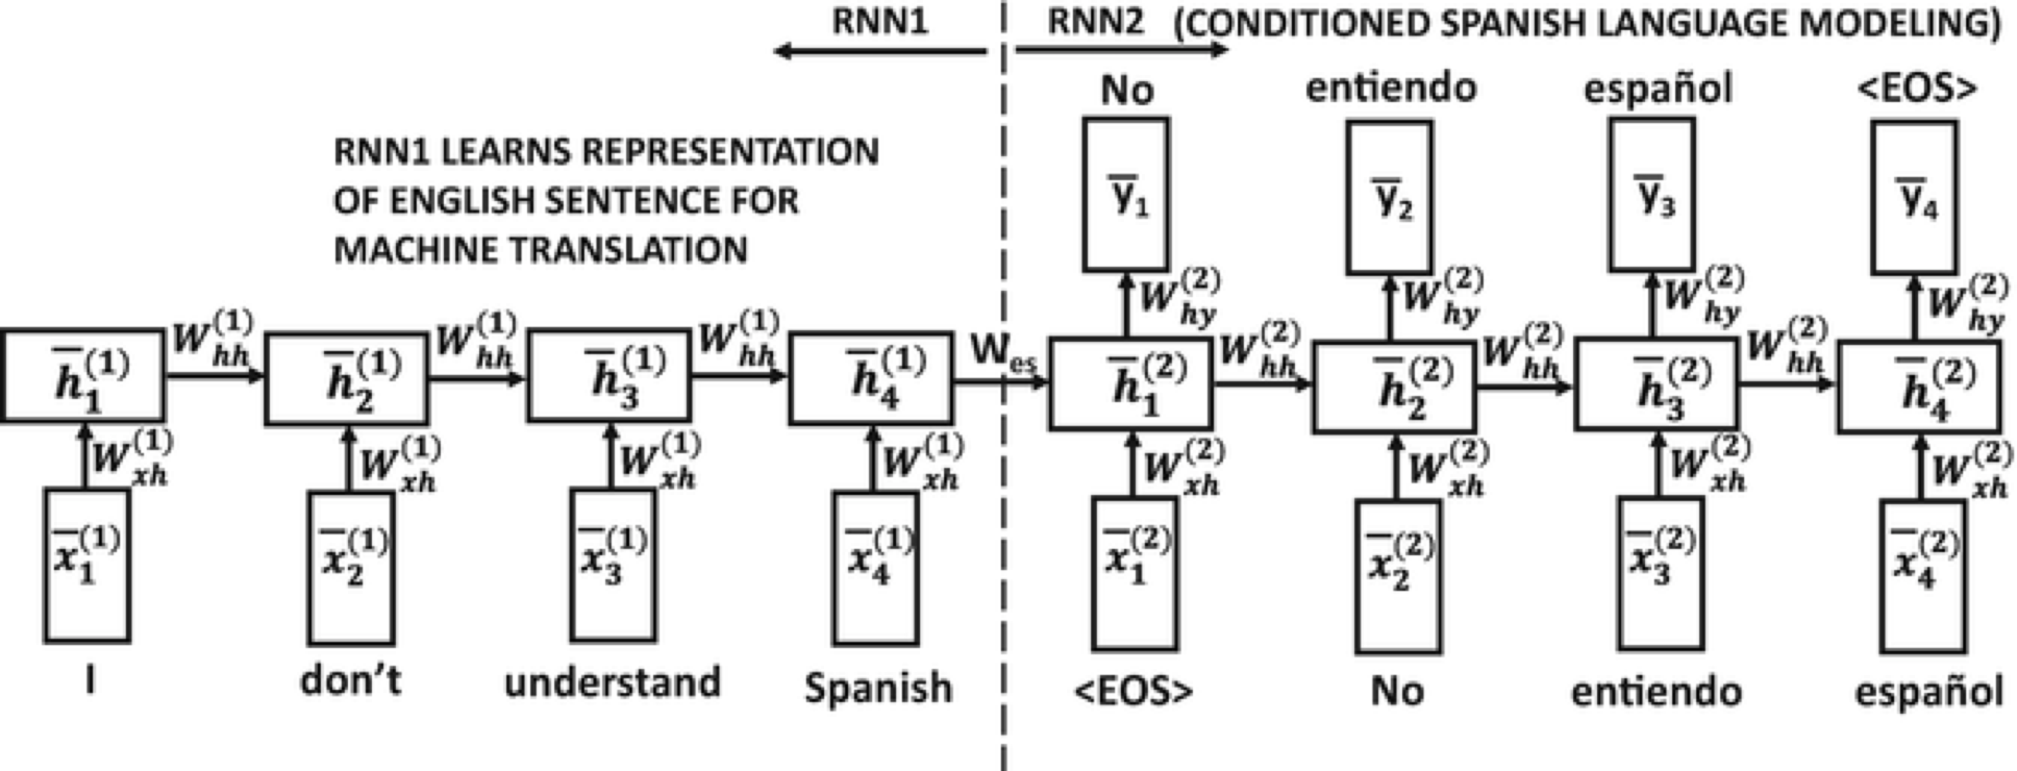
\includegraphics[width=\textwidth]{seq2seq.pdf}
\blfootnote{\url{https://link.springer.com/chapter/10.1007/978-3-319-73531-3_10}}

\end{frame}

\begin{frame}
\frametitle{Dynamic Attention Example - Seq2Seq models}
 
\begin{columns}
\begin{column}{0.3\textwidth}
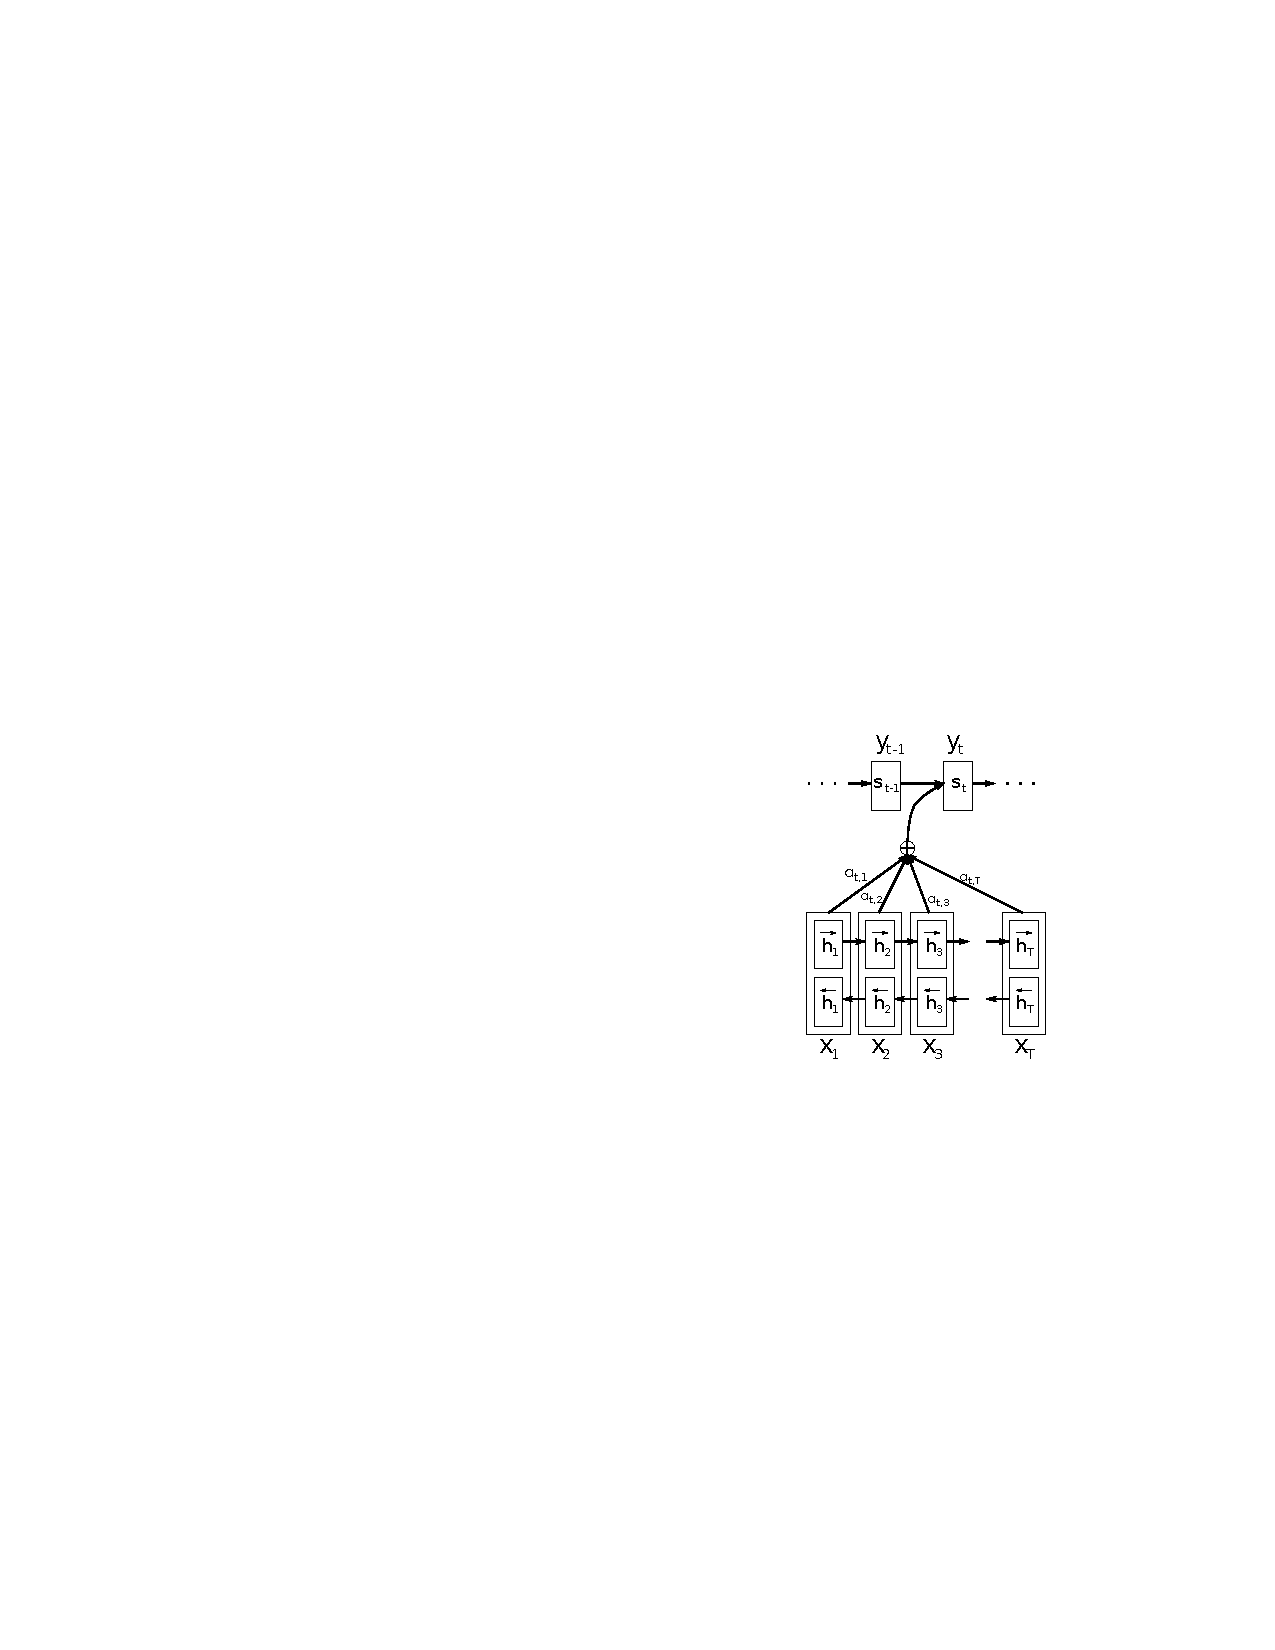
\includegraphics[width=\columnwidth]{context-attention.pdf}
\end{column}
\begin{column}{0.7\textwidth}
\[
\alpha_t = \softmax([\score(\vs_{t-1}, \vh_1), \dotsc, \score(\vs_{t-1}, \vh_T)]^\top)
\]
\[
\score(\vs, \vh) = \vv^\top \tanh{(\mW [\vs ; \vh])}
\]
\[
c = \alpha_t^\top \mH \text{ where } \mH = [h_1, h_2, \dotsc, h_T]^T
\]
\footnotesize{commonly known as ``Additive Attention'', even though it is based on concatenation!}
\end{column}
\end{columns}
\blfootnote{Bahdanau, D., Cho, K. and Bengio, Y., 2014. Neural machine translation by jointly learning to align and translate. ICLR 2015.}
\end{frame}



\begin{frame}
\frametitle{Hard Attention vs Soft-attention}
 
\begin{itemize}
  \item Soft-attention: use the softmax to smoothly attend mostly to one thing (but capture a bit of everything else)
  \item Hard attention: you specifically only attend to one thing: tricks (e.g. policy gradients or ST operator) from last lecture required to learn
\end{itemize}

\end{frame}

\begin{frame}
\frametitle{Aside: Relaxation of a map/hashtable/dictionary}
 

\end{frame}

\begin{frame}[t]
\frametitle{Scaled dot-product attention}

\[
\Attention(\mQ, \mK, \mV) = \softmax(\frac{\mQ\mK^\top}{\sqrt{d_k}})\mV
\]

\begin{itemize}
  \item<+-> In the previous Seq2Seq example we could replace additive attention with scaled dot-product attention with something like $\mQ = f(\vs_{t-1})$, $\mK = g(\mH)$ and $\mV = j(\mH)$.
  \item<+-> The scaling $1/\sqrt{d_k}$ is just to improve learning (larger $d_k$ implies larger dot products, which pushes further towards the flatter bit of the softmax, and thus smaller gradients.)
\end{itemize}

 
\end{frame}


\begin{frame}
\frametitle{Scaled dot-product self-attention}

\[
\SelfAttention(\mX) = \softmax(\frac{\mQ\mK^\top}{\sqrt{d_k}})\mV
\]
\[
\mQ = \mW_q \mX
\]
\[
\mK = \mW_k \mX
\]
\[
\mV = \mW_v \mX
\]

 
\end{frame}

\begin{frame}
\frametitle{Multi-head Attention}


\center
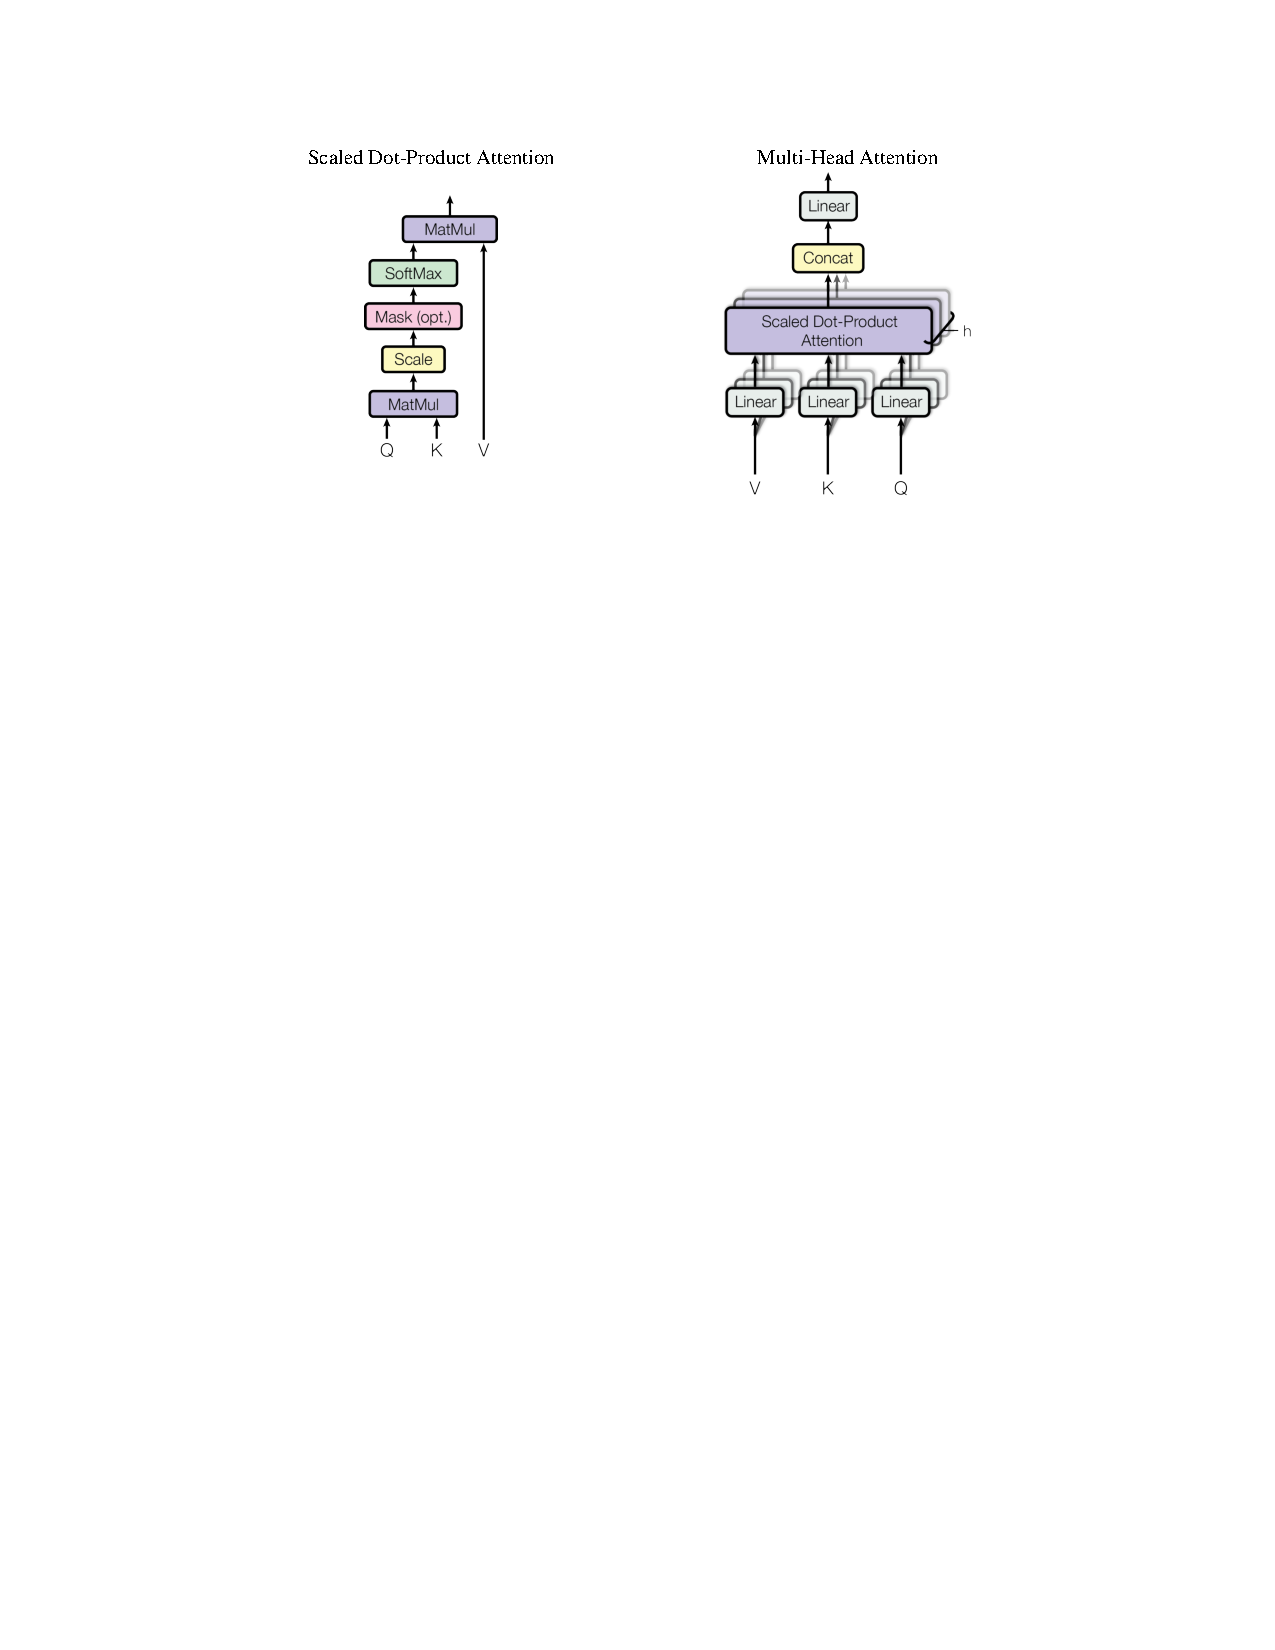
\includegraphics[width=0.75\textwidth]{multihead.pdf} \vspace{-1em}
\[
\MultiHead(\mQ, \mK, \mV) = [\mathrm{head}_1; \dots; \mathrm{head}_n]\mW^O
\]
\[
\mathrm{head}_i = Attention(QW_i^Q, KW_i^K, VW_i^V)
\]

\blfootnote{A. Vaswani, N. Shazeer, N. Parmar, J. Uszkoreit, L. Jones, A. N. Gomez, L. u. Kaiser, and I. Polosukhin. Attention is all you need. In Advances in Neural Information Processing Systems, volume 30.}
 
\end{frame}


\begin{frame}
\frametitle{The Transformer}
\center
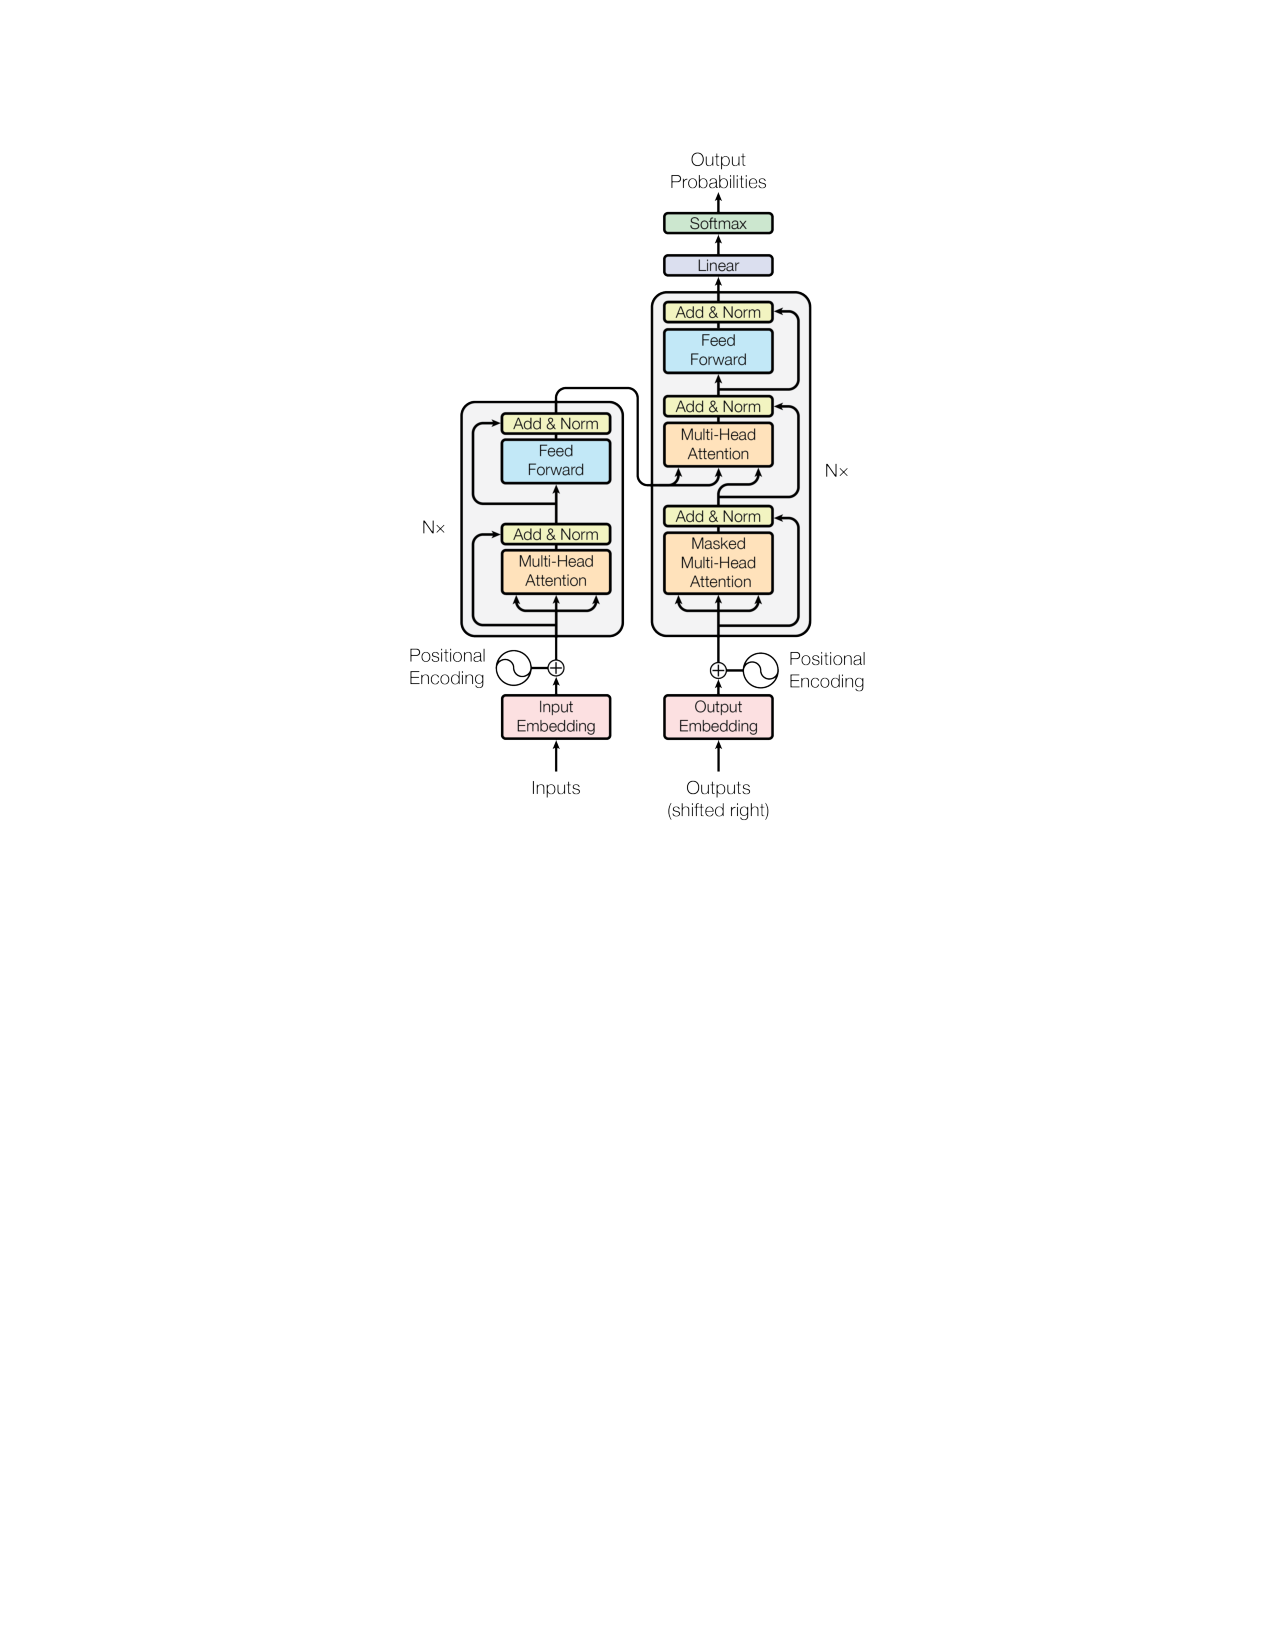
\includegraphics[scale=0.7]{transformer.pdf}
\end{frame}
\end{document}